\documentclass[a4paper]{jsarticle}
\setlength{\topmargin}{-20.4cm}
\setlength{\oddsidemargin}{-10.4mm}
\setlength{\evensidemargin}{-10.4mm}
\setlength{\textwidth}{18cm}
\setlength{\textheight}{26cm}

\usepackage[top=15truemm,bottom=25truemm,left=20truemm,right=20truemm]{geometry}
\usepackage[latin1]{inputenc}
\usepackage{amsmath}
\usepackage{amsfonts}
\usepackage{amssymb}
\usepackage[dvipdfmx]{graphicx}
\usepackage[dvipdfmx]{color}
\usepackage{listings}
\usepackage{listings,jvlisting}
\usepackage{geometry}
\usepackage{framed}
\usepackage{color}
\usepackage[dvipdfmx]{hyperref}
\usepackage{ascmac}
\usepackage{enumerate}
\usepackage{tabularx}
\usepackage{cancel}
\usepackage{scalefnt}

\renewcommand{\figurename}{fig.}
\renewcommand{\tablename}{table }
\newcommand{\redunderline}[1]{\textcolor{BrickRed}{\underline{\textcolor{black}{#1}}}} 

\hypersetup{
	colorlinks=false, % リンクに色をつけない設定
	bookmarks=true, % 以下ブックマークに関する設定
	bookmarksnumbered=true,
	pdfborder={0 0 0},
	bookmarkstype=toc
}

\lstset{
basicstyle={\ttfamily},
identifierstyle={\small},
commentstyle={\smallitshape},
keywordstyle={\small\bfseries},
ndkeywordstyle={\small},
stringstyle={\small\ttfamily},
frame={tb},
breaklines=true,
columns=[l]{fullflexible},
xrightmargin=0zw,
xleftmargin=3zw,
numberstyle={\scriptsize},
stepnumber=1,
numbersep=1zw,
lineskip=-0.5ex
}

\setcounter{tocdepth}{3}

\author{}
\title{機械力学}
\date{}

\begin{document}
\maketitle
\tableofcontents
\newpage

\section{一自由度並進運動}
\begin{itembox}[l]{運動方程式}
    \begin{eqnarray*}
        m\ddot{x}\left(t\right)+c\dot{x}\left(t\right)+kx\left(t\right)=F\left(t\right)\\
    \end{eqnarray*}
\end{itembox}
\section{剛体円盤のねじり振動系}
\begin{itembox}[l]{運動方程式}
    \begin{eqnarray*}
        I\ddot{\theta}\left(t\right)+c_\theta\dot{\theta}\left(t\right)+k_\theta\theta\left(t\right)&=&M\left(t\right)\\
    \end{eqnarray*}
\end{itembox}
\section{(例題) 回転に関する運動方程式を求める}
\begin{figure}[htbp]
    \begin{center}
        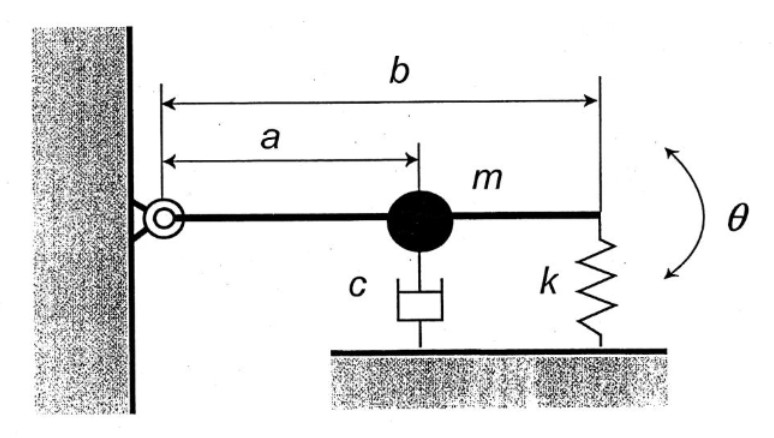
\includegraphics[width=100mm]{images/kiriki_image2.jpg}
        \caption{H18 試験問題 [3]}
    \end{center}
\end{figure}
\begin{itembox}[l]{Point}
    \begin{center}
        \textgt{(モーメント) = (発生する力) $\times$ (腕の長さ)}\\
        運動方程式に\textgt{腕の長さの二乗}が項に出てくる
    \end{center}
\end{itembox}
\begin{enumerate}[(1)]
    \item 質点について\\
          \begin{eqnarray*}
              (質点にはたらくモーメント)&=& [質点にはたらく力] \times (腕の長さ)\\
              &=& [(質量) \times (腕の長さ) \times (角加速度)] \times (腕の長さ)\\
              &=& m \times a \times \ddot{\theta}\left(t\right) \times a\\
              &=&ma^2\ddot{\theta}\left(t\right)
          \end{eqnarray*}
    \item ダッシュポットについて
          \begin{eqnarray*}
              (ダッシュポットにはたらくモーメント)&=& [ダッシュポットにはたらく力] \times (腕の長さ)\\
              &=& [(減衰係数) \times (腕の長さ) \times (角速度)] \times (腕の長さ)\\
              &=& m \times a \times \dot{\theta}\left(t\right) \times a\\
              &=&ca^2\dot{\theta}\left(t\right)
          \end{eqnarray*}
    \item ばねについて
          \begin{eqnarray*}
              (ばねにはたらくモーメント)&=& [ばねにはたらく力] \times (腕の長さ)\\
              &=& [(ばね定数)) \times (腕の長さ) \times (回転角)] \times (腕の長さ)\\
              &=& m \times b \times \theta\left(t\right) \times b\\
              &=&kb^2\dot{\theta}\left(t\right)
          \end{eqnarray*}
\end{enumerate}
以上の(1),(2),(3)より,回転に関する運動方程式は
\begin{eqnarray*}
    ma^2\ddot{\theta}\left(t\right)+ca^2\dot{\theta}\left(t\right)+kb^2\dot{\theta}\left(t\right)=0\\
\end{eqnarray*}
\section{自由振動}
外力がゼロのとき,自由振動という.\\
このとき,運動方程式の右辺はゼロとなり,そのときの応答は2階の同次微分方程式を解くことで求めることができる.
\begin{itembox}[l]{Point}
    \begin{eqnarray*}
        (固有振動数\;\omega)&=&(減衰のない系の自由振動の振動数)\\
        (減衰固有振動数\;\omega_d)&=&(減衰のある系の自由振動の振動数(減衰自由振動数))\\
    \end{eqnarray*}
\end{itembox}
\begin{itembox}[l]{固有振動数}
    \begin{eqnarray*}
        \omega_n = \sqrt{\dfrac{k}{m}}\\
    \end{eqnarray*}
\end{itembox}
\begin{itembox}[l]{減衰比}
    \begin{eqnarray*}
        \zeta = \dfrac{c}{2\sqrt{mk}}\\
    \end{eqnarray*}
\end{itembox}
\begin{itembox}[l]{減衰固有振動数}
    \begin{eqnarray*}
        \omega_d&=&\sqrt{1-\zeta^2}\omega_n\\
    \end{eqnarray*}
\end{itembox}
\begin{itembox}[l]{振動数と周期}
    \begin{eqnarray*}
        \omega=\dfrac{2\pi}{T}\\
    \end{eqnarray*}
\end{itembox}
\section{特性方程式}
運動方程式(自由振動)に$\; x\left(x\right)=e^{st}\;$を代入して整理すると,以下のような\textgt{特性方程式}を得ることができる.
\begin{itembox}[l]{特性方程式}
    \begin{eqnarray*}
        s^2+2\zeta\omega_ns+\omega_n^2=0\\
    \end{eqnarray*}
\end{itembox}
これを満たす$\; s_1,s_2\;$の組を\textgt{特性根}という.
\subsection{過減衰}
$\zeta>1$のとき,特性根は
\begin{eqnarray*}
    s_1,s_2=\left(-\zeta \pm \sqrt{\zeta^2-1}\right)\omega_n
\end{eqnarray*}
の相異なる負の実数となる.
したがって,応答$x\left(t\right)$は以下のようになる.
\begin{itembox}[l]{過減衰の応答}
    \begin{eqnarray*}
        x\left(t\right)=a_1\exp{\left(s_1t\right)}+a_2\exp{\left(s_2t\right)}\\
    \end{eqnarray*}
\end{itembox}
ここで,$t\rightarrow\infty$で$0$に漸近する.
そのため,振動は繰り返しを伴わない.($\neq$振動)\\
このとき,これを\textgt{過減衰}という.
\subsection{臨界減衰}
$\zeta = 0$のとき,特性根は
\begin{eqnarray*}
    s_1=s_2=-\omega_n
\end{eqnarray*}
したがって,応答$x\left(t\right)$は以下のようになる.
\begin{itembox}[l]{臨界減衰の応答}
    \begin{eqnarray*}
        x\left(t\right)=a_1\exp{\left(-\omega_nt\right)}+a_2t\exp{\left(-\omega_nt\right)}\\
    \end{eqnarray*}
\end{itembox}
このときの応答を\textgt{臨界減衰}といい,応答の収束が最も速くなる.
\subsection{不足減衰}
$0<\zeta<1$のとき,特性根は
\begin{eqnarray*}
    s_1,s_2=\left(-\zeta \pm i\sqrt{1-\zeta^2}\right)\omega_n\\
\end{eqnarray*}
の共役な複素数となる.
したがって,応答$x\left(t\right)$は以下のようになる.(導出省略)
\begin{itembox}[l]{不足減衰の応答}
    \begin{eqnarray*}
        x\left(t\right)&=&A\exp{\left(-\zeta \omega_nt\right)}\cos{\left(\sqrt{1-\zeta^2}\omega_nt\right)}+B\exp{\left(-\zeta \omega_nt\right)}\sin{\left(\sqrt{1-\zeta^2}\omega_nt\right)}\\
        x\left(t\right)&=&A\exp{\left(-\zeta \omega_nt\right)}\cos{\left(\omega_dt\right)}+B\exp{\left(-\zeta \omega_nt\right)}\sin{\left(\omega_dt\right)}\\
        \\
        x\left(t\right)&=&C\exp{\left(-\zeta \omega_nt\right)}\cos\left(\sqrt{1-\zeta^2}\omega_nt+\varphi\right)
    \end{eqnarray*}
    \begin{eqnarray*}
        \omega_d=\sqrt{1-\zeta^2}\omega_n\;&:&\;減衰固有振動数\\
        \varphi\;&:&\;位相角\\
        ※ A,B,C&&は任意定数\\
    \end{eqnarray*}
\end{itembox}
\begin{itembox}[l]{三角関数の合成}
    \begin{eqnarray*}
        a\sin\theta+b\cos\theta
        &=&\sqrt{a^2+b^2}\left(\dfrac{a}{\sqrt{a^2+b^2}}\sin\theta+\dfrac{b}{\sqrt{a^2+b^2}}\cos\theta\right)\\
        &=&\sqrt{a^2+b^2}\left(\sin\theta\dfrac{a}{\sqrt{a^2+b^2}}+\cos\theta\dfrac{b}{\sqrt{a^2+b^2}}\right)\\
        &=&\sqrt{a^2+b^2}\left(\sin\theta\cos\alpha+\cos\theta\sin\alpha\right)\\
        &=&\sqrt{a^2+b^2}\sin\left(\theta+\alpha\right)\\
        \\
        a\sin\theta+b\cos\theta
        &=&\sqrt{a^2+b^2}\left(\dfrac{a}{\sqrt{a^2+b^2}}\sin\theta+\dfrac{b}{\sqrt{a^2+b^2}}\cos\theta\right)\\
        &=&\sqrt{a^2+b^2}\left(\cos\theta\dfrac{b}{\sqrt{a^2+b^2}}+\sin\theta\dfrac{a}{\sqrt{a^2+b^2}}\right)\\
        &=&\sqrt{a^2+b^2}\left(\cos\theta\cos\alpha+\sin\theta\sin\alpha\right)\\
        &=&\sqrt{a^2+b^2}\cos\left(\theta-\alpha\right)\\
        \\
        ※\quad\tan\alpha &=& -\dfrac{b}{a}
    \end{eqnarray*}
\end{itembox}
\subsection{単振動}
$\zeta = 0$のとき,特性根は
\begin{eqnarray*}
    s_1,s_2=i\omega_n\\
\end{eqnarray*}
の共役な純虚数となる.
したがって,応答$x\left(t\right)$は以下のようになる.(導出省略)
\begin{itembox}[l]{単振動の応答}
    \begin{eqnarray*}
        x\left(t\right)&=&A\cos{\omega_nt}+B\sin{\omega_nt}\\
    \end{eqnarray*}
\end{itembox}
このとき,減衰係数$\zeta=0$より,いつまでも減衰しない\textgt{単振動}となる.\\
\\
ここで,極の実部(負になる)は\textgt{自由振動の減衰の速さ}を表し,極の虚部は\textgt{自由振動の振動数}を表している.
\section{強制振動}
\textgt{強制振動}とは,外力が存在する振動である.\\
このとき,運動方程式の右辺に外力$f\left(t\right)$の項を持ち,その応答は
重ね合わせの原理から右辺がゼロの自由振動における2階の同次微分方程式の一般解に,
特殊解を足し合わせることで求めることができる.\\
\section{調和外力に対する定常応答}
\begin{itembox}[l]{調和外力}
    \begin{center}
        周期性を持つ外力のことを\textgt{調和外力}という.$\sin$波や$\cos$波に相当する.
    \end{center}
\end{itembox}
\begin{itembox}[l]{定常応答}
    \begin{center}
        加振開始から十分な時間が経過した後の応答を\textgt{定常応答}といい,運動方程式の\textgt{特殊解}に相当する.\\
        また,そのような状況を\textgt{定常状態}という.定常応答解析では初期時刻という概念を考えない.\\
        外力は無限の過去に始まり,未来永劫続いている
    \end{center}
\end{itembox}
\subsection{三角関数による方法}
定常応答を求めるには,
\begin{eqnarray*}
    m \ddot{x}\left(t\right)+c\dot{x}\left(t\right)+kx\left(t\right)=f\cos\omega t
\end{eqnarray*}
を解けばよい.(ここでは,外力を$f\left(t\right)=f\cos\omega t$)としている.\\
外力$f\left(t\right)$が\textgt{振動数$\omega$をもつ繰り返し力}であることから,
それに駆動される定常応答もまた\textgt{同じ振動数を持つ繰り返し}になるはずである.
ただし,\textgt{振幅}(振動の大きさ)と\textgt{位相}(山谷のタイミング)は異なる可能性がある.\\
ここで,振幅$x_0$と外力に対する位相遅れ$\varphi$を未知量として,特殊解の形を$x\left(t\right)=x_0\cos\left(\omega t-\varphi\right)$
と\textgt{予想する}して,運動方程式に代入し$\cos\varphi,\sin\varphi$について整理すると
\begin{eqnarray*}
    x_0\cos\varphi&=&\dfrac{-m\omega^2+k}{\left(-m\omega^2+k\right)^2+\left(c\omega\right)^2}f\\
    x_0\sin\varphi&=&\dfrac{c\omega}{\left(-m\omega^2+k\right)^2+\left(c\omega\right)^2}f
\end{eqnarray*}
したがって,振幅$x_0$は,
\begin{itembox}[l]{振幅$x_0$}
    \begin{eqnarray*}
        x_0=\sqrt{\left(x_0\cos\varphi\right)^2+\left(x_0\sin\varphi\right)^2}=\dfrac{1}{\sqrt{\left(-m\omega^2+k\right)^2+\left(c\omega\right)^2}}f\\
    \end{eqnarray*}
\end{itembox}
位相遅れ$\varphi$は,$x_0\cos\varphi,x_0\sin\varphi$の比をとったものであるので,
\begin{itembox}[l]{位相遅れ$\varphi$}
    \begin{eqnarray*}
        \varphi=\mathrm{Tan}^{-1}\left(\dfrac{x_0\sin\varphi}{x_0\cos\varphi}\right)=\mathrm{Tan}^{-1}\left(\dfrac{c\omega}{-m\omega^2+k}\right)\\
    \end{eqnarray*}
\end{itembox}
\subsection{複素振幅表示による方法(1)}
\begin{itembox}[l]{Point}
    \begin{eqnarray*}
        f\left(t\right)
        &=&Fe^{i\omega t}\\
        &=&A\cos\left(\omega t\right)+Bi\sin\left(\omega t\right)\\
        &=&|F|\sin\left(\omega t -\varphi_1\right)\\
        &=&|F|\cos\left(\omega t -\varphi_2\right)\\
        \\
        f\left(t\right) &が& \sin\; の項を持つ場合\; \rightarrow \; A=0\\
        f\left(t\right) &が& \cos\; の項を持つ場合\; \rightarrow \; B=0\\
    \end{eqnarray*}
\end{itembox}
三角関数を用いて考えたときと同様に外力を$f\left(t\right)=f\cos\omega t$とする.
\begin{eqnarray*}
    x\left(t\right)&=&Xe^{i\omega t}\\
    f\left(t\right)&=&Fe^{i\omega t}\\
    ※\quad\omega &:& 外力の振動数
\end{eqnarray*}
を代入することで,三角関数を用いる方法より簡単に応答の振幅,位相遅れを求めることができる.\\
ここで,$X$を\textgt{複素振幅}といい,$|X|$は\textgt{振動振幅}$x_0$を,
$-\angle X$は\textgt{位相遅れ}$\varphi$を表す.\\
\begin{itembox}[l]{Point}
    \begin{center}
        \textgt{複素振幅}を用いることで,\textgt{振動振幅}と\textgt{位相遅れ}の2つの情報を1つの関数で表すことができる
    \end{center}
\end{itembox}
以上の式を,運動方程式に代入して整理すると,\\
\begin{eqnarray*}
    \left(-m\omega^2+ic\omega+k\right)Xe^{i\omega t}=Fe^{i\omega t}\\
\end{eqnarray*}
となることから,複素振幅$X$,振動振幅$|X|$,位相遅れ$\varphi$は,
\begin{itembox}[l]{複素振幅$X$}
    \begin{eqnarray*}
        X=\dfrac{F}{-m\omega^2+ic\omega+k}\\
    \end{eqnarray*}
\end{itembox}
\begin{itembox}[l]{振動振幅$|X|$}
    \begin{eqnarray*}
        x_0=|X|&=&\dfrac{F}{\sqrt{\left(-m\omega^2+k\right)^2+\left(c\omega\right)^2}}\\
    \end{eqnarray*}
\end{itembox}
\begin{itembox}[l]{位相遅れ$\varphi$}
    \begin{eqnarray*}
        \varphi=-\angle X &=&\mathrm{Tan}^{-1}\left(\dfrac{c\omega}{-m\omega^2+k}\right)\\
    \end{eqnarray*}
\end{itembox}
定常応答$x\left(t\right)$は,
\begin{eqnarray*}
    x\left(t\right)&=&x_0\cos\left(\omega t-\varphi\right)\\
\end{eqnarray*}
に上記の値を代入したものになる.\\
\subsection{複素振幅表示による方法(2)}
つぎに,固有振動数$\omega_n$,減衰比$\zeta$を用いて考える.\\
このとき,運動方程式は以下のように書き換えることができる.
\begin{eqnarray*}
    \ddot{x}\left(t\right)+2\zeta\omega_n\dot{x}\left(t\right)+\omega_n^2 x\left(t\right)=\frac{f}{m}\cos\omega t
\end{eqnarray*}
同様に,以下の式を運動方程式に代入して整理すると,
\begin{eqnarray*}
    x\left(t\right)&=&Xe^{i\omega t}\\
    f\left(t\right)&=&Fe^{i\omega t}\\
    ※\quad\omega &:& 外力の振動数\\
    ※\quad F &=& \frac{f}{m}
\end{eqnarray*}
\begin{eqnarray*}
    \left(-\omega^2+2\zeta\omega_n\omega i+\omega_n^2\right)Xe^{i\omega t}=Fe^{i\omega t}\\
\end{eqnarray*}
となることから,複素振幅$X$,振動振幅$|X|$,位相遅れ$\varphi$は,
\begin{itembox}[l]{複素振幅$X$}
    \begin{eqnarray*}
        X=\dfrac{F}{-\omega^2+2\zeta\omega_n\omega i+\omega_n^2}\\
    \end{eqnarray*}
\end{itembox}
\begin{itembox}[l]{振動振幅$|X|$}
    \begin{eqnarray*}
        x_0=|X|&=&\dfrac{F}{\sqrt{\left(\omega_n^2-\omega^2\right)^2+\left(2\zeta\omega_n\omega\right)^2}}\\
    \end{eqnarray*}
\end{itembox}
\begin{itembox}[l]{位相遅れ$\varphi$}
    \begin{eqnarray*}
        \varphi=-\angle X &=&\mathrm{Tan}^{-1}\left(\dfrac{2\zeta\omega_n\omega}{\omega_n^2-\omega^2}\right)\\
    \end{eqnarray*}
\end{itembox}
定常応答$x\left(t\right)$は,
\begin{eqnarray*}
    x\left(t\right)&=&x_0\cos\left(\omega t-\varphi\right)\\
\end{eqnarray*}
に上記の値を代入したものになる.\\
※ 調和振動が $\sin$ の項を持つ場合は,$\cos$から$\sin$に変えれば良い.
\subsection{周波数応答関数$G_f$}
$X/F$の絶対値は外力の振幅に対する応答の\textgt{振幅比}を,偏角に負号をつけたものは外力に対する応答の位相遅れを表す.
ここで,$G_f=X/F$とおくと,$G_f$は$\omega$の関数になり,これを\textgt{周波数応答関数}という.
\begin{itembox}[l]{周波数応答関数}
    \begin{eqnarray*}
        G_f\left(\omega\right)=\dfrac{X}{F}=\dfrac{1}{-m\omega^2+ic\omega +k}\\
    \end{eqnarray*}
\end{itembox}
周波応答関数は,\textgt{単位大きさの正弦波外力に対する定常応答の複素振幅}を,\textgt{外力の振動数(加振振動数)}の関数としてあらわしたものである.
\begin{itembox}[l]{振幅比$|X/F|$}
    \begin{eqnarray*}
        \left|\dfrac{X}{F}\right|=|G_f\left(\omega\right)|=\dfrac{1}{-m\omega^2+ic\omega+k}\\
    \end{eqnarray*}
\end{itembox}
\begin{itembox}[l]{位相遅れ$\varphi$}
    \begin{eqnarray*}
        \varphi=-\angle X &=&\tan^{-1}\left(\dfrac{c\omega}{-m\omega^2+k}\right)\\
    \end{eqnarray*}
    \begin{center}
        ※ 複素振幅の位相遅れと同じ
    \end{center}
\end{itembox}
\section{共振曲線}

\section{その他}
\subsection{合成ばね定数を求める}
系の平衡状態から,力を加えたと仮定して力のつり合いを考えることで合成ばね定数を求めることができる.
\begin{itembox}[l]{Point}
    \begin{center}
        (\textgt{質点に加わる力})\quad=\quad(\textgt{合成ばね定数})\quad×\quad(\textgt{変位の合計})
    \end{center}
\end{itembox}
※ 質点に加わる力は,「$f$」等で適当におくと良い.(後々消える)

\end{document}